\section{Ejercicio FR - Trayectoria en 3D}

\subsection{Problema}

Represente la trayectoria de la partícula en el espacio tridimensional y analice los resultados.

Presente en una misma gráfica el comportamiento de tres velocidades adimensionales (extraídas de la anterior simulación) en función del tiempo medido en nanosegundos. En concreto, se pide el módulo de la velocidad del electrón relativista en función del tiempo, el componente $v_z$ de su velocidad y su velocidad radial $v_r = \sqrt{ v_x^2 + v_y^2}$. 

\subsection{Resolución}

\paragraph{Gráfica de $\vec{r}(t)$} 
Primero mostramos la posición de la partícula.

\begin{figure}[H]
	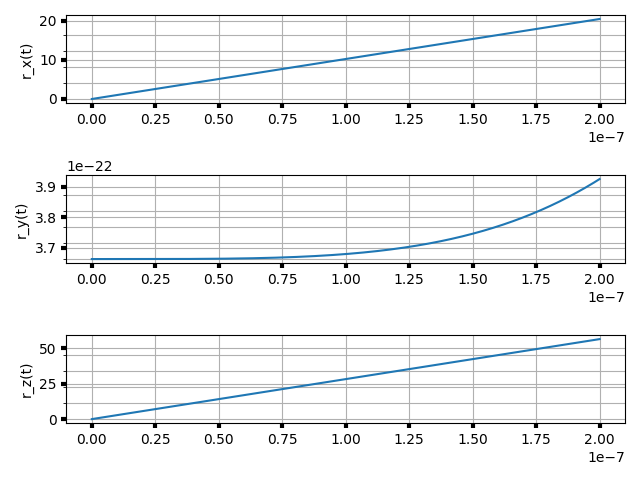
\includegraphics[width=\linewidth]{figures/rel_rx_ry_rz.png}
	\caption{Gráfica $r_x(t)$, $r_y(t)$, $r_z(t)$ en función de $t$}
	\label{fig:rel_rx_ry_rz_t}
\end{figure}

\newpage 

\paragraph{Gráfica de $\frac{\vec{v}(t)}{c}$}

Ahora mostramos una gráfica de $\vec{v}(t)$ adimensionada por $c$.

\begin{figure}[H]
	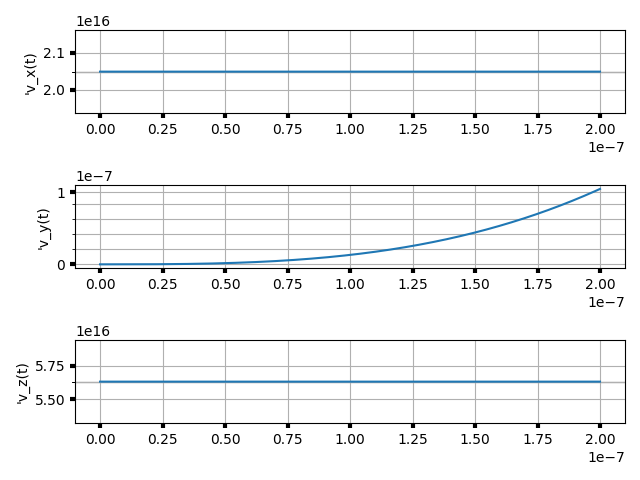
\includegraphics[width=\linewidth]{figures/rel_adim_vx_vy_vz.png}
	\caption{Gráfica $\vec{v}(t)$ adimensionada}
	\label{fig:rel_adim_vx_vy_vz}
\end{figure}

